\section{\label{II_3_A}Reversement des données au sein du FRBR} 

Le processus automatisé proposé repose sur l'exécution de deux phases : d'une part la segmentation temporelle d'un flux vidéo (géérant des time codes et des images-clé), et d'autre part la détection et la classification d'objets (générant des mots-clés). L'enjeu est de prévoir la structuration de ces différents types de données, chiffrées et textuelles, au sein du modèle FRBR existant. 

%Certains outils ont déjà été développés dans d’autres applications de gestion des collections afin d’effectuer ce reversement de manière automatique : Wedia, Keepeek, Einden, MomaSoft “classent automatiquement les images et vidéos en leur attribuant les métadonnées appropriées.” \footcite{zotero-item-732}

Les outils automatiques utilisés lors du processus ont extrait des données depuis un média, associé au niveau de l'item numérique au sein du modèle de données préexistant. Or, le niveau item contient des éléments de description matérielle techniques, alors que les mots-clés et repères temporels relèvent d'une description intelectuelle et syntaxique. Dès lors, la création d'une entité intelectuelle dédiée à la séquence s'impose. 
Afin d'illustrer l'intégration d'une entité de description intermédiaire, entre l'oeuvre et l'item numérique, prenons l'exemple de la plateforme Okapi (Open and Knowledge-based Annotation and Publishing Interface), développée par le département Recherche et Innovation de l'\gls{ina} \footcite{lalande2022}. Afin de favoriser la description collaborative de contenus multimédias, la plateforme offre la possibilité aux utilisateurs de concevoir des modèles de description personnalisés \footcite{lalande2022}. La plateforme permet notamment de séparer l'extrait audiovisuel du média, dont il constitue un niveau descriptif propre. Une strate supplémentaire de description est ainsi dédiée à la description intellectuelle du média. Le modèle FRBR tel que nous l'avons décrit ne propose, a priori, pas d'entité descriptive dédiée à la séquence. L'entité "d'agrégats", proposée par le manuel de la \gls{fiaf} pourrait y correspondre. Toutefois, ceux-ci “sont conçus et créés dès le début pour rassembler plusieurs composantes individuelles formant un tout." \footcite{zotero-item-646}. Or, au sein du corpus étudié, les rushes ne font pas partie d'un montage. Toute segmentation est une interprétation a posteriori de la construction de l’archive, et donc un remontage. L'entité de "fragment d'expression" proposé par l'IFLA au sein du modèle FRBR bibliographique semble plus adéquate \footcite{iflastandards.info2026}. L’\gls{IFLA} définit le fragment comme “des parties d’expressions qui ne constituent pas elles-mêmes des expressions autonomes.[...] Un « Fragment d’expression » n’est identifié qu’en fonction de son occurrence au sein d’un tout connu ou supposé.” \footcite{iflastandards.info2026}. Cette entité semble correspondre à la notion de séquences telle que nous l'avons décrite. Elle serait rattachée à l’Oeuvre, conformément à l’adaptation du FRBR par les recommandations de la FIAF, et permettrait le reversement spécifique des times-codes et mots-clés. La figure \ref{figfragment} ci-dessous illustre l'intégration de l'entité du fragment d'oeuvre au modèle de données existant. 

\begin{figure}[htbp] 
	
	\centering 
	
	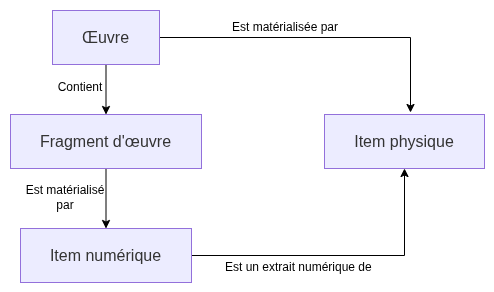
\includegraphics[width=0.7\textwidth]{images/fragment_frbr.png} 
	
	\caption{Intégration du Fragment au modèle de données} 
	
	\label{figfragment} 
	
\end{figure} 

Au sein de la plateforme Okapi, la création d'une entité intermédiaire de description, permet aux données descriptives produites à partir du média, d'être reversées au sein d'un niveau parent essentiellement descriptif, celui de l'extrait. Au sein du modèle de données existant, adapté au corpus étudié, les time codes et les mots-clés sont déjà indexés manuellement en tant que données au sein de l’application. En effet, les times codes sont renseignés au niveau de l'item numérique, dans un champ notes, et l'item comporte le champ type renseigné par la valeur “fichier time codé”, afin de signifier sa qualité d'extrait. De plus, les mots-clés sont renseignés au niveau de l’indexation de l’œuvre, donc du rush original. La modélisation de la segmentation au sein du modèle actuel implique un nombre conséquent de relations entre les éléments, complexifiant ainsi la navigation de l'utilisateur. En effet, une notice d'item physique renseigne tous les extraits numériques (items numériques) qui lui sont liés. L’item numérique (segment) renseigne le film physique duquel il est extrait, tandis que le niveau œuvre renseigne uniquement les extraits numériques qui lui sont associés. 
La création d’une nouvelle entité simplifierait la navigation au sein de l'interface et permettrait de séparer la description en différents niveaux, intellectuel et technique, conformément aux principes du FRBR. La nouvelle entité de fragments permettrait éventuellement de préciser un contexte de segmentation et des champs dédiés aux mots clés et aux time codes. Le tableau \ref{tab:reversement_metadonnees_frbr} ci-dessous illustre la répartition de la description entre le fragment d'Oeuvre et l'item numérique. Pour des raisons de clarté, d'autres données descriptives ont été intégrées afin d'illustrer la répartition entre la description intellectuelle et matérielle. 

\begin{table}[H]
	\centering
	\small
	\renewcommand{\arraystretch}{1.3}
	\begin{tabular}{|p{3.8cm}|p{4.2cm}|p{6.4cm}|}
		\hline
		\textbf{Entité FRBR} & \textbf{Champ / Attribut} & \textbf{Exemples de valeurs} \\
		\hline
		\multirow{6}{=}{\textbf{Fragment d’Oeuvre} \newline \textit{(Description intellectuelle)}} 
		& Contexte & Segmentation automatique de tel item physique \\ \cline{2-3}
		& Description générale & Description du contenu sémantique de la séquence \\ \cline{2-3}
		& Processus de segmentation & Automatique (Outil utilisé et paramètres appliqués) \\ \cline{2-3}
		& Time codes & Time codes de début et de fin de la séquence \\ \cline{2-3}
		& Mots-clés & Mots-clés extraits par YOLO \\ \cline{2-3}
		& Image-clé associée & Lien direct vers le fichier de l'image-clé \\ \cline{2-3}
		& Oeuvre parente & Identifiant de l'oeuvre associée, lien direct vers la notice \\ \cline{2-3}
		& Item physique associé & Identifiant de l'item physique associé dont est tirée la séquence, lien direct vers la notice \\ \cline{2-3}
		& Item numérique associé & Identifiant de l'item numérique associé, lien direct vers la notice \\ 
		\hline
		\multirow{3}{=}{\textbf{Item Numérique} \newline \textit{(Description technique et matérielle)}} 
		& Fragment associé & Identifiant du fragment associé, lien direct vers la notice \\ \cline{2-3}
		& Données techniques & Résolution de l'image, taille, format \\ \cline{2-3}
		& Données de conservation & Emplacement, contenant \\ \cline{2-3}
		& Média associé & fichier média de la séquence \\ \cline{2-3}
		\hline
	\end{tabular}
	\caption{Attributs et exemples de valeurs associées aux entités Fragment d'Expression et Item Numérique.}
	\label{tab:reversement_metadonnees_frbr}
\end{table}

Les métadonnées automatiquement produites seraient intégrées au niveau du fragment, tandis que l'item numérique contiendrait le média et les données techniques. 
Une difficulté subsiste toutefois. En effet, les processus s'exécutent au niveau du fichier numérique et de son média, tandis que les métadonnées produites doivent pouvoir enrichir un niveau descriptif supérieur, celui du fragment. Dexu configurations peuvent être envisagées afin d'opérer ce reversement automatiquement. D'une part, l'application gère actuellement l'héritage des données d'un niveau supérieur à un niveau inférieur via la configuration de méta-masques, qui ciblent les niveaux iférieurs au sein desquels reverser les données. Néanmoins, le processus automatisé décrit impliquerait la configuration de masques ascendants, permettant de reverser des métadonnées générées au niveau de l'item, vers l'entité de fragment. Cette configuration complexifie toutefois la compréhension du modèle de données.
D'autre part, pourrait être envisagé la mise en place d'un tableau de correspondance ou d'un script permettant d'associer les sorties de données du processus aux entités dans lesquelles elles doivent être injectées. 
Une fois la modélisation du transfert établie entre les métadonnées automatiquement produites, et le modèle de données existant, le reversement définitif est toutefois laissé à l'utilisateur métier, au sein de l'interface du logiciel. 
%À l’ingest : données interdépendantes entre la description d’un item numérique et de son média. Mentionner la relation nouvelle sur l’item numérique et son média : facilite les choses pour le reversement  
%Pour les times codes, des champs dédiés devrons être prévus sous le champ film associé.  
%Faire un schéma de métadonnées pour pouvoir adapter les données aux normes du logiciel via des connecteurs par exemple.  
